\chapter{Proposta}
\label{cap:proposta}

Nesta seção é detalhada são detalhadas as etapas de coleta de dados, pré-processamento e processamento que envolvem o desenvolvimento do modelo de percepção veicular de ambiente e propriocepção veicular.

\section{Captação de Dados}

Uma vez que não foram encontrados \textit{datasests} disponibilizando publicamente dados de sensores inerciais e de sensores auxiliares neste contexto de STIs, foram realizadas diversas coletas de dados. Sendo assim, foram criados 9  \textit{datasests} nomeados \textit{Passive Vehicular Sensors Dataset} (PVS 1-9), reunindo dados de diversos sensores de abordagem passiva. Para a coleta de dados, foram utilizadas duas redes de sensores, sendo cada uma delas constituídas por um Single-Board Computer (SBC) Raspberry Pi e três placas MPU-9250, cada uma equipada com um acelerômetro, um giroscópio, um magnetômetro e um sensor de temperatura. Também foi utilizado uma fonte externa de GPS, com produção de dados de localização e velocidade, além de uma câmera para captura de vídeo ambiente. A Tabela \ref{table:sensor_network_hardware} detalha o hardware utilizado.

\begin{table}[h!]
\small
\caption{Hardware da rede de sensores.} 
\label{table:sensor_network_hardware}
\centering
\begin{tabular}{llll}
\toprule
\multicolumn{1}{l}{\textbf{Hardware}} & 
\multicolumn{1}{l}{\textbf{Sensor}} & 
\multicolumn{1}{l}{\textbf{Dado}} & 
\multicolumn{1}{l}{\textbf{Taxa}}  
\\ \midrule

\multicolumn{1}{l}{HP Webcam HD-4110} & 
\multicolumn{1}{l}{Câmera} & 
\multicolumn{1}{l}{720p Video} & 
\multicolumn{1}{c}{30 Hz}                   
\\ \midrule

\multicolumn{1}{l}{Xiaomi Mi 8} & 
\multicolumn{1}{l}{GPS} & 
\multicolumn{1}{l}{Velocidade em m/s, latitude, longitude, etc.} &
\multicolumn{1}{c}{1 Hz}
\\ \midrule

\multicolumn{1}{l}{\multirow{5}{*}{MPU-9250}} & 
\multicolumn{1}{l}{Acelerômetro} & 
\multicolumn{1}{l}{Aceleração em 3 eixos ($m/s^2$)} &
\multicolumn{1}{c}{\multirow{5}{*}{100 Hz}} 
\\ \cmidrule(lr){2-3}

\multicolumn{1}{l}{} & 
\multicolumn{1}{l}{Giroscópio} & 
\multicolumn{1}{l}{Taxa de rotação em 3 eixos (deg/s)} & 
\multicolumn{1}{l}{}                       
\\ \cmidrule(lr){2-3}

\multicolumn{1}{l}{} & 
\multicolumn{1}{l}{Magnetômetro} & 
\multicolumn{1}{l}{Campo geomagnético ambientam em 3 eixos ($\mu T$)} & 
\multicolumn{1}{l}{}
\\ \cmidrule(lr){2-3}

\multicolumn{1}{l}{} & 
\multicolumn{1}{l}{Temperatura} &
\multicolumn{1}{l}{Temperatura do sensor em $^{\circ}C$} & 
\multicolumn{1}{l}{}                       
\\ \bottomrule

\end{tabular}
\end{table}

Todo o equipamento de hardware foi fixado no veículo. A câmera foi colocada no lado externo do teto, e o receptor de GPS foi colocado internamente, na dashboard. As duas redes com as placas MPU-9250 foram distribuídas no veículo de forma a considerar os dados provindos de pontos com diferentes influências da propriedade de dependência veicular. Sendo assim, cada extremidade do eixo frontal (lado direito e esquerdo) recebeu uma das redes, onde anexou-se uma placa na bandeja da suspensão, localizando-se abaixo e próximo à suspensão veicular; outra placa acima e próxima à suspensão, anexada na lataria; e outra placa anexada na dashboard do veículo, dentro da cabine. Em relação ao referencial de captação das placas MPU-9250, utilizou-se posicionamento controlado, onde o colocação das placas foi realizada de forma que os três eixos do sistema de coordenadas do sensor são alinhados com os do veículo sendo, portanto, tanto referencial de captação como de análise. O acelerômetro foi configurado com full scale select de 8g \footnote{1g = 9.8 $m/s^2$} e o giroscópio com 1000 deg/s (propriedade sensorial).

Uma vez que este trabalho objetiva o desenvolvimento de um modelo que considera os fatores de dependência, além da amostragem de velocidade (propriedade de condução) e do posicionamento dos sensores inerciais em diferentes pontos do veículo (propriedade veicular), é necessário a produção de dados em contextos distintos, para se obter uma variabilidade de cenários para validar o modelo. Sendo assim, o conjunto de sensores detalhados acima foi utilizado em três veículos diferentes (propriedade veicular), com três condutores diferentes (propriedade de condução) percorrendo três cenários distintos (propriedade ambiental), onde em cada um há três diferentes tipos de superfície, além de variações gerais do ambiente, como presença de lombadas, buracos, condição de conservação do pavimento, etc. A Tabela \ref{table:datasets_description} detalha o contexto de cada dataset.

\begin{table}[h!]
\small
\caption{Descrição dos datasets.} 
\label{table:datasets_description}
\centering
\begin{tabular}{llllllllll}
\toprule
\textbf{Dataset} & PVS 1 & PVS 2 & PVS 3 & PVS 4 & PVS 5 & PVS 6 & PVS 7 & PVS 8 & PVS 9 
\\ \midrule
\textbf{Veículo} & 
\multicolumn{3}{l}{Volkswagen Saveiro} & 
\multicolumn{3}{l}{Fiat Bravo} & 
\multicolumn{3}{l}{Fiat Palio}
\\ \midrule
\textbf{Motorista} & 
\multicolumn{3}{l}{Motorista 1} & 
\multicolumn{3}{l}{Motorista 2} & 
\multicolumn{3}{l}{Motorista 3} 
\\ \midrule
\textbf{Cenário} & 1  & 2  & 3  & 1 & 2 & 3 & 1 & 2 & 3 
\\ \bottomrule
\end{tabular}
\end{table}

\begin{figure}[h!]
  \centering
  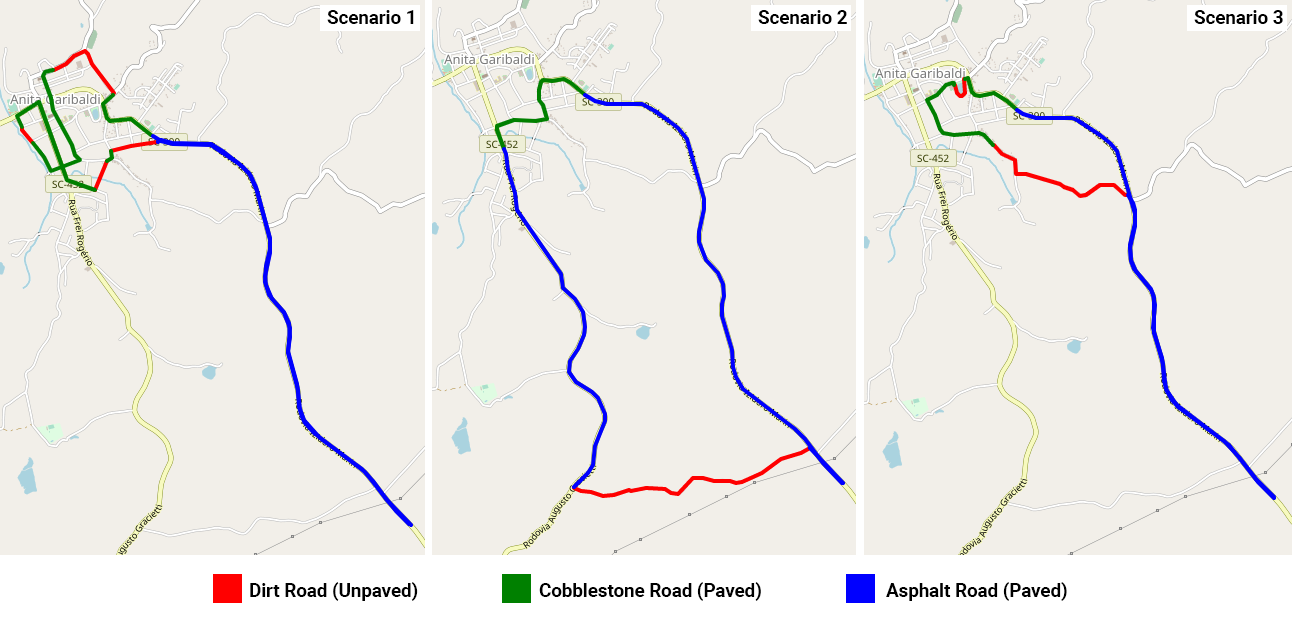
\includegraphics[width=1\textwidth]{figuras/scenarios.png}
  \caption{Cenários de coleta de dados.}
  \label{fig:data_collection_scenarios}
\end{figure}

Em relação ao tipo de superfície de pista, cada cenário possui trechos do trajeto em sem pavimentação (terra) e pavimentados (paralelepípedo ou asfalto). A Figura \ref{fig:data_collection_scenarios} ilustra cada cenário, e a Figura \ref{fig:data_collection_surface_types} ilustra as superfícies. A Tabela \ref{table:datasets_metrics} quantifica as amostras e distâncias. Os dados foram amostrados na cidade de Anita Garibaldi, em Santa Catarina, Brasil, entre os dias 24 e 26 de dezembro de 2019. Os códigos-fonte utilizados na coleta de dados, para manipulação de sensores, amostragem e armazenamento dos sinais; no pré-processamento, com ajustes, combinação de dados, normalização, etc.; no processamento, com a classificação dos padrões; assim como os próprios datasets, estão documentados e disponíveis no github para pesquisas futuras \footnote{https://github.com/Intelligent-Vehicle-Perception}.

\begin{figure}[h!]
  \centering
  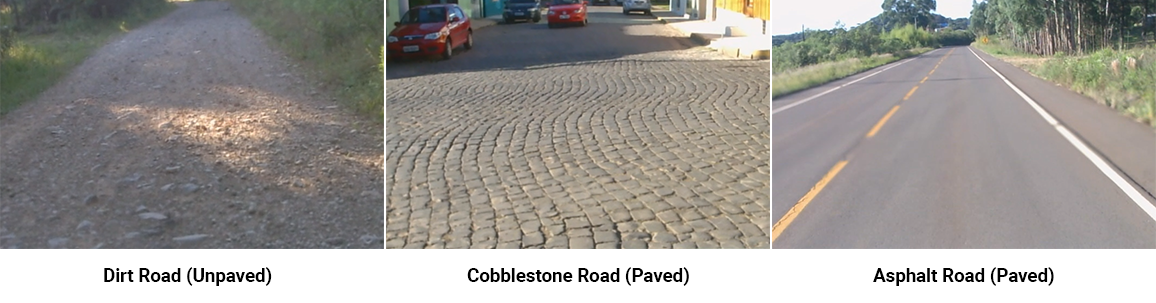
\includegraphics[width=1\textwidth]{figuras/surface_type.png}
  \caption{Tipos de superfícies nos cenários.}
  \label{fig:data_collection_surface_types}
\end{figure}

\begin{table}[h!]
\small
\caption{Métricas dos datasets.} 
\label{table:datasets_metrics}
\begin{tabular}{cccccccccc}
\cmidrule(l){3-10} & & 
\multicolumn{4}{c}{\textbf{Amostras (nº)}} & 
\multicolumn{4}{c}{\textbf{Distância (km)}} 
\\ \midrule

\multicolumn{1}{c}{\textbf{Cenário}} &
\textbf{Dataset} &
\textbf{\begin{tabular}[c]{@{}c@{}}Terra\end{tabular}} &
\textbf{\begin{tabular}[c]{@{}c@{}}Paralele-\\pípedo\end{tabular}} &
\textbf{\begin{tabular}[c]{@{}c@{}}Asfalto\end{tabular}} & 
\textbf{Total} &
\textbf{\begin{tabular}[c]{@{}c@{}}Terra\end{tabular}} &
\textbf{\begin{tabular}[c]{@{}c@{}}Paralele-\\pípedo\end{tabular}} &
\textbf{\begin{tabular}[c]{@{}c@{}}Asfalto\end{tabular}} & 
\textbf{Total} 
\\ \midrule

\multicolumn{1}{c}{\multirow{4}{*}{1}} & 
PVS 1 & 
25868 & 61659 & 56509 & 144036 & 
1.59 & 3.53 & 8.7 & 13.81
\\ \cmidrule(l){2-10} 

\multicolumn{1}{c}{} & 
PVS 4 & 
23903 & 57670 & 50919 & 132492 & 
1.58 & 3.51 & 8.72 & 13.81
\\ \cmidrule(l){2-10} 

\multicolumn{1}{c}{} & 
PVS 7 & 
23778 & 54224 & 50546 & 128548 & 1.59 & 3.49 & 8.69 & 13.78
\\ \midrule

\multicolumn{1}{c}{\multirow{4}{*}{2}} & 
PVS 2 & 
44618 & 20737 & 59330 & 124684 & 
2.17 & 1.39 & 8.07 & 11.62 
\\ \cmidrule(l){2-10} 

\multicolumn{1}{c}{} & 
PVS 5 & 
60539 & 18143 & 55195 & 133877 & 
2.16 & 1.38 & 8.09 & 11.63 
\\ \cmidrule(l){2-10} 

\multicolumn{1}{c}{} &
PVS 8 & 
44939 & 18825 & 59854 & 123618 & 
2.16 & 1.37 & 8.09 & 11.63 
\\ \midrule

\multicolumn{1}{c}{\multirow{4}{*}{3}} & 
PVS 3 & 
28659 & 26143 & 51014 & 105816 & 
1.66 & 1.66 & 7.4 & 10.72 
\\ \cmidrule(l){2-10} 

\multicolumn{1}{c}{} & 
PVS 6 & 
23888 & 31641 & 40750 & 96279 & 
1.38 & 1.93 & 7.43 & 10.73 
\\ \cmidrule(l){2-10} 

\multicolumn{1}{c}{} & 
PVS 9 & 
23153 & 25182 & 43220 & 91555 & 
1.67 & 1.66 & 7.42 & 10.74 
\\ \bottomrule
\end{tabular}
\end{table}

\section{Pré-Processamento}

Após a coleta, os dados brutos foram pré-processados antes de serem parametrizados para as técnicas de Machine Learning, de acordo com as etapas ilustradas na Figura \ref{fig:pre_processing_steps}. Inicialmente foram realizados ajustes nos dados, como combinação de dados dos sensores inerciais com os do GPS, onde para cada cada amostra do MPU-9250 foi associada a última localização e velocidade conhecida. Também foram criados vídeos de plotagem dos sinais, disponíveis no github, os quais sincronizados com o vídeo ambiente auxiliaram na criação dos rótulos de tipo de superfície na forma one-hot-encoded. Sendo assim, este estudo conta com Ground-Truth (GT) humano.

\begin{figure}[h!]
  \centering
  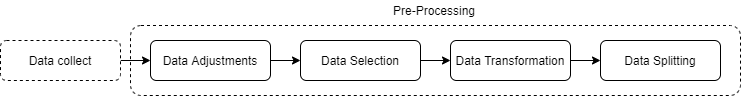
\includegraphics[width=1\textwidth]{figuras/pre-processing.png}
  \caption{Etapas de pré-processamento.}
  \label{fig:pre_processing_steps}
\end{figure}

Após os ajustes iniciais, foram selecionados os dados a serem utilizados. Neste estudo focou-se na utilização dos valores amostrados na bandeja da suspensão, localizado abaixo e próximo a sistema de suspensão. Estes valores são menos influenciados pela propriedade de dependência veicular, de acordo com o modelo Quarter Car (QC), sendo afetados pela rigidez do pneu e por sua capacidade de absorção \cite{Yafeai2019}. Sendo assim, cada amostra utilizada possuí os valores de aceleração em três eixos, a taxa de rotação em três eixos, e a velocidade. Neste estudo, considerou-se todos os eixos e não apenas o de maior interesse, como geralmente é feito em estudos de percepção de ambiente com sensores inerciais, uma vez que todos os eixos apresentam informações importantes, que devem ser consideradas no desenvolvimento de um modelo de maior precisão e acurácia.

Com os dados selecionados, estes foram transformados para se adequarem às entradas das técnicas de classificação de padrões. Para os métodos de Classical Machine Learning, foi realizada a extração de características dos dados com métodos estatísticos de desvio padrão, média e variância para os sensores inerciais, e média para a velocidade, consistindo dos métodos mais comumente utilizados em estudos relacionados para extração de características de alto nível baseadas em dados de vibração de sinais de sensores inerciais \cite{Alqudah2016, Andria2016, BelloSalau2018, Bose2018, Hou2017, Li2016, Lima2016, Pholprasit2015, Prapulla2017, Savera2016, Singh2017}. Para analisar a influência da quantidade de amostras, foram utilizadas janelas de 100, 150, 200, 250 e 300 amostras, considerando 100 o tamanho mínimo para se ter informações suficientes, e 300 o tamanho máximo para que o delay da primeira classificação não seja maior que 3 segundos. Para os métodos de Deep Learning, os dados foram normalizados com robust scaler, min-max scaler (0,1) e min-max scaler (-1,1), uma vez que estas técnicas produzem melhor desempenho quando as variáveis de entrada e saída são dimensionadas em uma faixa de valores. Após, os dados também foram agrupados em janelas de mesmo tamanho das técnicas clássicas.

Após a transformação dos dados, foram definidos quais seriam utilizados para treinamento e quais para validação. Embora comumente um dataset seja dividido em uma parte para treinamento e outra para validação, no contexto deste estudo este tipo de particionamento incorre em viés por dois motivos. O primeiro, se todos os datasets tiverem uma parte para treinamento e outra para validação, isto implica que a técnica de reconhecimento de padrões terá como dados de treinamento todos os veículos, com todos os motoristas em todos os cenários. Isto, por si só, já leva a técnica a obter excelentes resultados, mas não nos diz nada a respeito da capacidade de generalizar sua classificação de padrões em cenários não conhecidos. Em segundo, este tipo de particionamento pode levar a situações em que os dados de validação são constituído majoritariamente por dados de com padrões mais facilmente reconhecidos, como os padrões de pavimentação asfáltica, uma vez que a vibração nos sinais deste tipo de superfície é muito menor que nas demais. Sendo assim, para que se possa avaliar corretamente a capacidade de generalização das técnicas, avaliando sua confiabilidade em cenários desconhecidos, optou-se por realizar a divisão de dados de treinamento e validação de acordo com o dataset, separados em três experimentos específicos:\newline

\textbf{Experimento 1:}
\begin{itemize}
    \item \textbf{Treinamento (65\%):} PVS 1, PVS 3, PVS 4, PVS 6, PVS 7, PVS 9. 
    \item \textbf{Validação (35\%):} PVS 2, PVS 5, PVS 8.
    \item \textbf{Descrição:} A técnica aprende todos os veículos, mas não todos os cenários.\newline
\end{itemize}

\textbf{Experimento 2:}
\begin{itemize}
    \item \textbf{Treinamento (66\%):} PVS 1, PVS 2, PVS 3, PVS 7, PVS 8, PVS 9.
    \item \textbf{Validação (34\%):} PVS 4, PVS 5, PVS 6.
    \item \textbf{Descrição:} A técnica aprende todos os cenários, mas não todos os veículos.\newline
\end{itemize}

\textbf{Experimento 3:}
\begin{itemize}
    \item \textbf{Treinamento (66\%):} PVS 1, PVS 2, PVS 4, PVS 6, PVS 8, PVS 9.
    \item \textbf{Validação (34\%):} PVS 3, PVS 5, PVS 7.
    \item \textbf{Descrição:} A técnica aprende alguns cenários e alguns veículos, mas não todos os cenários para todos os veículos.
\end{itemize}

\section{Processamento}

\subsection{Classificação de Tipo de Superfície de Pista}

Para a classificação de padrões de tipo de superfície de pista, duas abordagens foram empregadas, visando identificar a mais apropriada, sendo técnicas de Classical Machine Learning e de de Deep Learning. A Figura \ref{fig:processing_steps} detalha as abordagens e métodos. Nas seções seguintes são detalhadas as abordagens e técnicas desenvolvidos.

\begin{figure}[h!]
  \centering
  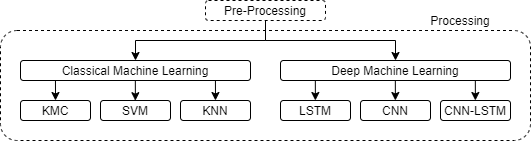
\includegraphics[width=0.8\textwidth]{figuras/processing.png}
  \caption{Abordagens e técnicas para classificação.}
  \label{fig:processing_steps}
\end{figure}

\subsubsection{Machine Learning Clássico}

Diversas técnicas clássicas de Machine Learning foram utilizadas em trabalhos relacionados a percepção de ambiente com sinais de sensores inerciais \cite{menegazzo2018}. Para aplicação destes métodos, ao contrário da abordagem de Deep Learning, foi necessário realizar em pré-processamento a extração de características de alto nível dos dados brutos, que representem bem os padrões que se deseja reconhecer \cite{Goodfellow2016}. Dentre os métodos com esta abordagem mais aplicados na área, estão os três experimentados neste estudo: K-Means Clustering (KMC), Support Vector Machines (SVM) e K-Nearest Neighbors (KNN). Para a técnica de KMC, os modelos foram definidos com o número de 3 clusters, representando as classes de tipo de superfície que se pretende identificar. Para o KNN, de forma a identificar o valor ótimo de vizinhos para este estudo, experimentou-se modelos com 1, 2, 5, 10, 50, 100, 250, 500, 1000 vizinhos. Já para SVM, foram analisados modelos para 3 kernels, sendo polinomial de grau 3, rbf e sigmoid.

\subsubsection{Deep Learning}

Nos estudos de percepção veicular com sensores inerciais, poucos utilizam desta abordagem para reconhecer padrões em sinais de vibração, não sendo encontrado nenhum que aplique estas técnicas ao problema deste trabalho. Sendo assim, as Deep Neural Networks (DNN) desenvolvidas foram baseadas em estudos de reconhecimento de atividade humana \cite{Deep2019, Alemayoh2019, Chen2015, Yang2018, Zebin2018, Zebin2019, Wang2019, Ahmad2019}, estimativa de velocidade de caminhada \cite{Shrestha2018} e classificação de tipos de terreno durante a corrida \cite{Dixon2019}. Foram analisados modelos baseados em LSTM, baseados em CNN e baseados em CNN-LSTM. Todos os modelos desenvolvidos utilizam o otimizador Adam em conjunto com a função de perda categorical cross entropy, uma vez que se trata de um problema de classificação multi classe. 

Para a abordagem LSTM-based, foram experimentados diversos modelos de rede, dentre Vanilla LSTM e Stacked LSTM, ambas na forma unidirecionais e bidirecionais, detalhados na Tabela \ref{table:lstm_models}. 

\small
\begin{longtable}{cl}
\caption{Modelos DNN baseados em LSTM..} 
\label{table:lstm_models} \\
\toprule \textbf{name} & \multicolumn{1}{c}{\textbf{layers}} \\ \midrule
\endfirsthead
\toprule \textbf{name} & \multicolumn{1}{c}{\textbf{layers}} \\ \midrule
\endhead \endfoot \endlastfoot
LSTM 1 & \begin{tabular}[c]{@{}l@{}}
1 LSTM with 100 units, 1 Dropout of 0.5, 1 Dense of 100 units and relu activation, \\ 1 Dense with 3 units and softmax activation.
\end{tabular} \\ \midrule
LSTM 2 & Same as LSTM 1, but connecting LSTM returned sequences flattened directly to Dense block. \\ \midrule
LSTM 3 & Same as LSTM 1, but LSTM are bidirectional. \\ \midrule
LSTM 4 & Same as LSTM 2, but LSTM are bidirectional. \\ \midrule
LSTM 5 & \begin{tabular}[c]{@{}l@{}}
3 blocks of LSTM with 100 units and Dropout 0.5, 1 Dense with 100 units and relu activation, \\ 1 Dense with 3 units and softmax activation.
\end{tabular} \\ \midrule
LSTM 6 & Same as LSTM 5, but LSTM are bidirectional and Dropout 0.2 \\ \midrule
LSTM 7 & \begin{tabular}[c]{@{}l@{}}
3 blocks of LSTM with 100 units, Batch Normalization and Dropout 0.5, \\ 1 Dense with 100 units and relu activation, 1 Dense with 3 units and softmax activation.\end{tabular} \\ \bottomrule
\end{longtable}

O modelo desenvolvido com melhores resultados foi o LSTM 7, de uma Stacked LSTM Unidirecional detalhado na Figura \ref{fig:lstm_dnn}. Neste modelo, a DNN recebe de entrada um tensor rows x sequences x channels, onde rows é a quantidade de janelas, as sequences são as janelas de dados, e os channels são as 7 variáveis dos sensores. O modelo é composto de uma camada de entrada, três blocos de recorrência e regularização, e um bloco de camadas fully connected para produção da saída. As camadas LSTM de 100 unidades são usadas para aprender s dependências temporais de longo prazo entre as etapas de tempo dos dados de sequência. A regularização é feita por duas camadas, sendo as de Batch Normalization para padronizar as entradas de uma nova camada, reduzindo o tempo de treinamento \cite{Zebin2018} e melhorando o desempenho; e Dropout em 50\% para evitar o overfitting ignorando neurônios selecionados aleatoriamente durante o treinamento. Após o processamento nas camadas recorrentes, os parâmetros vão para duas camadas Dense, a primeira de 100 neurônios com ativação Relu, e a segunda com 3 neurônios de ativação Softmax, produzindo a classificação esperada. Como saída esperada da rede, foi utilizada os labels correspondentes a última amostra da janela.

\begin{figure}[h!]
  \centering
  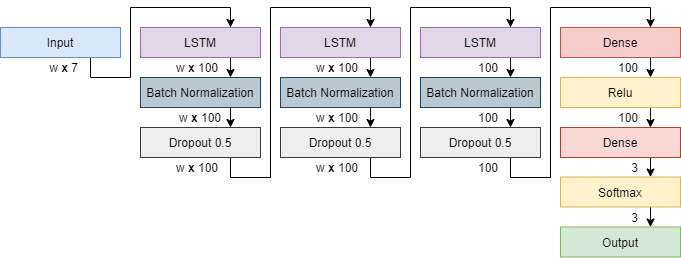
\includegraphics[width=1\textwidth]{figuras/lstm_dnn.png}
  \caption{Melhor DNN baseada em LSTM.}
  \label{fig:lstm_dnn}
\end{figure}

Para a abordagem baseada em CNN, foram experimentados modelos de CNN Stacked, com utilização de diferentes camadas de pooling, conforme detalha a Tabela \ref{table:cnn_models}.

\small
\begin{longtable}{cl}
\caption{Modelos DNN baseados em CNN.} 
\label{table:cnn_models} \\
\toprule \textbf{name} & \multicolumn{1}{c}{\textbf{layers}} \\ \midrule
\endfirsthead
\toprule \textbf{name} & \multicolumn{1}{c}{\textbf{layers}} \\ \midrule
\endhead \endfoot \endlastfoot
CNN 1 & \begin{tabular}[c]{@{}l@{}}
3 blocks of Conv1D with 64-64-128 filters, kernel 3 and relu activation, 1 Flatten, \\ 
1 Dense with 100 units and relu activation, 1 Dense with 3 units and softmax activation.
\end{tabular} \\ \midrule
CNN 2 & Same as CNN 1, but with a max pooling 1D of pool size 2 after the convolution blocks. \\ \midrule
CNN 3 & \begin{tabular}[c]{@{}l@{}}
1 Conv1D with 64 filters, kernel 3 and relu activation, 1 Batch Normalization, 1 Dropout\\ 
0.15, 1 Conv1D with 32 filters, kernel 3 and relu activation, 1 Global Avg Pool 1D, 1 Batch \\ 
Normalization, 1 Dropout 0.2 and 1 Dense with 3 units and softmax activation.
\end{tabular} \\ \midrule
CNN 4 & \begin{tabular}[c]{@{}l@{}}
2 Conv1D with 100 filters, kernel 10 and relu activation, 1 Max Pooling 1D with pool size 3\\ 
2 Conv1D with 160 filters, kernel 10 and relu activation, 1 Global Avg Pool 1D, 1 Dropout 0.5\\ 
and 1 Dense with 3 units and softmax activation.
\end{tabular} \\ \midrule
CNN 5 & \begin{tabular}[c]{@{}l@{}}
1 Conv1D with 64 filters, kernel 3 and activation relu, 1 Max Pooling 1D with pool size 2, \\ 
1 Conv1D with 64 filters, kernel 3 and activation relu, 1 Flatten and 1 Dense with 3 units \\
and softmax activation.
\end{tabular} \\ \midrule
CNN 6 & \begin{tabular}[c]{@{}l@{}}
1 Conv1D with 24 filters, kernel 8 and activation relu, 1 Batch Normalization, 1 Spatial \\ 
Dropout 0.15, 1 Conv1D with 12 filters, kernel 8 and activation relu, 1 Global Avg Pool 1D, \\
1 Batch Normalization, 1 Dropout 0.2, 1 Dense with 48 units and relu activation, 1 Batch \\
Normalization, Dropout 0.25, 1 Dense with 3 units and softmax activation.
\end{tabular} \\ \midrule
CNN 7 & \begin{tabular}[c]{@{}l@{}}
3 blocks of Conv1D with 128-64-32 filters, kernel 3, relu activation, Batch Normalization\\ 
and Max Pooling 1D with pool size 2, 1 Flatten, 1 Dropout 0.2, 1 Dense with 3 units and \\
softmax activation.
\end{tabular} \\ \midrule
\multicolumn{1}{l}{CNN 8} & \begin{tabular}[c]{@{}l@{}}
2 blocks of Conv1D with 64-32 filters, kernel 3, relu activation, Batch Normalization\\ 
and Dropout 0.15, 1 Conv1D 32 filters, kernel 3, relu activation, 1 Global Avg Pool 1D,\\ 1 Batch Normalization, 1 Dropout 0.2, 1 Dense with 32 units and relu activation and\\ 
1 Dense with 3 units and softmax activation.
\end{tabular} \\ \bottomrule
\end{longtable}

O modelo baseada em CNN desenvolvido com melhores resultados foi a CNN 8, detalhada na Figura \ref{fig:cnn_dnn}. A DNN recebe de entrada um tensor rows x windows x channels semelhante a baseada em LSTM, os quais são processados por três blocos de convolução e regularização, e um bloco de camadas fully connected. Os blocos de extração de características utilizam sobre os sinais kernels de convolução de tamanho 3, sendo o primeiro com 64 filtros, e os outros com 32 filtros. A regularização é feita pelas camadas de Batch Normalization e Dropout em 15\% e 20\%. O último bloco de extração de características conta ainda com uma camada de Global Average Pooling 1D para extrair características mais robustas através da média dos valores de cada região, acelerando o processo de treinamento e evitando overfitting \cite{Yang2018, Wang2019}. Por fim, o último bloco é composto por duas camadas Dense, uma com 32 neurônios e ativação Relu, e a outra 3 neurônios e Softmax. Como saída esperada da rede, foi utilizada os labels de maior frequência presentes na janela analisada. 

\begin{figure}[h!]
  \centering
  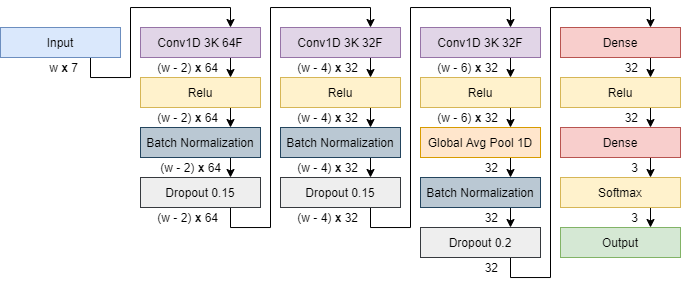
\includegraphics[width=1\textwidth]{figuras/cnn_dnn.png}
  \caption{Melhor DNN baseado em CNN.}
  \label{fig:cnn_dnn}
\end{figure}

Para a abordagem baseada em CNN-LSTM, foram experimentados os modelos detalhados na Tabela \ref{table:cnn_lstm_models}.

\small
\begin{longtable}{cl}
\caption{Modelos DNN baseados em CNN-LSTM.} 
\label{table:cnn_lstm_models} \\
\toprule \textbf{name} & \multicolumn{1}{c}{\textbf{layers}} \\ \midrule
\endfirsthead
\toprule \textbf{name} & \multicolumn{1}{c}{\textbf{layers}} \\ \midrule
\endhead \endfoot \endlastfoot
CNN-LSTM 1 & \begin{tabular}[c]{@{}l@{}}
2 Conv1D with 64 filters, kernel 3 and relu activation, 1 Dropout 0.5, 1 Max Pooling 1D \\ 
with pool size 2, 1 Flatten, 1 LSTM with 100 units, 1 Dropout 0.2, 1 Dense with 100 units \\ 
and relu activation, 1 Dense with 3 units and softmax activation
\end{tabular} \\ \midrule
CNN-LSTM 2 & Same as CNN-LSTM 1, but with 3 Conv1D layers. \\ \midrule
CNN-LSTM 3 & Same as CNN-LSTM 2, but with 3 blocks of LSTM and Dropout after the Max Pooling 1D. \\ \midrule
CNN-LSTM 4 & Same as CNN-LSTM 3, but LSTM blocks do not have Dropout. \\ \midrule
CNN-LSTM 5 & \begin{tabular}[c]{@{}l@{}}
2 blocks of Conv1D with 128 filters, kernel 3 and relu activation, Max Pooling 1D with \\ 
pool size 2 and Batch Normalization, 1 block of Conv1D with 128 filters, kernel 3 and relu \\ 
activation, Global Avg Pool 1D and Batch Normalization, 3 blocks of LSTM with 100 units, \\ 
Batch Normalization and Dropout 0.3, 1 Dense with 3 units and softmax activation.
\end{tabular} \\ \midrule
CNN-LSTM 6 & \begin{tabular}[c]{@{}l@{}}
2 blocks of Conv1D with 128 filters, kernel 3 and relu activation, Batch Normalization, and \\ 
Spatial Dropout 0.15, 1 block of Conv1D with 128 filters, kernel 3 and relu activation, Global \\ 
Avg Pool 1D, Batch Normalization and Dropout 0.2, 3 blocks of LSTM with 100 units, Batch \\ 
Normalization and Dropout 0.3, 1 Dense with 3 units and softmax activation.
\end{tabular} \\ \bottomrule
\end{longtable}

O modelo baseado em CNN-LSTM desenvolvido com melhores resultados foi o CNN-LSTM 6, detalhada na Figura \ref{fig:cnn_lstm_dnn}. A DNN recebe de entrada um tensor rows x sequences x subsequences x channels, onde as rows são a quantidade de janelas, sequences são as janelas de dados, subsequences são os subagrupamentos da janela, e channels as 7 variáveis dos sensores. Os dados são inicialmente processados por três blocos de convolução e regularização, três blocos de recorrência e regularização, e um bloco de camadas fully connected. Os blocos de extração de características utilizam sobre os sinais kernels de convolução de tamanho 3 e 128 filtros. A regularização é feita pelas camadas de Batch Normalization e Spatial Dropout 1D em 15\% e 20\%. O último bloco conta com uma camada de Global Average Pooling 1D. Em seguida, os blocos de recorrência possuem camadas de LSTM 100 units, e regularização por de Batch Normalization e Dropout 50\%. Por fim, os parâmetros resultantes são entregues a uma camada Dense com 3 neurônios e ativação Softmax, produzindo a classificação. Como saída esperada da rede, foi utilizada os labels correspondentes a última amostra da janela.

\begin{figure}[h!]
  \centering
  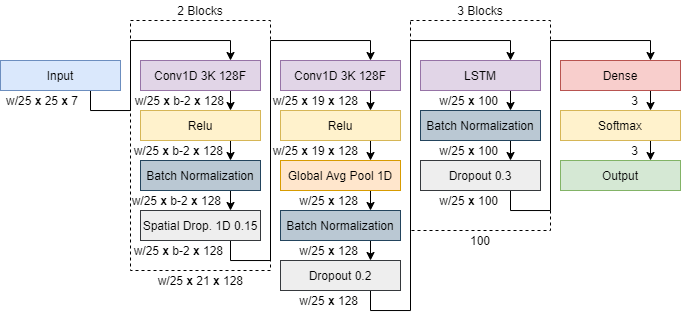
\includegraphics[width=1\textwidth]{figuras/cnn_lstm_dnn.png}
  \caption{Melhor DNN baseado em LSTM-CNN.}
  \label{fig:cnn_lstm_dnn}
\end{figure}
